\clearpage

\section{Evaluation}
\label{cp5:evaluation}



The goal of our evaluation is to assist the design of tools that use the explored techniques to help developers in locating text relevant to their task.
Therefore, evaluation focuses 
on determining what portion of the text identified by human annotators the techniques that we explore can automatically identify.
Experimental setup is as follows.



\subsubsection{Baseline}


As done by~\cite{Lin2021} and~\cite{Ye2016}, we use a standard \texttt{VSM} lexical similarity approach as a baseline. Our rationale to use 
lexical similarity as a baseline is based on the fact that 
both our card sorting analysis (\red{Chapter~\ref{aaa}}) and related work~\cite{Ko2006a, Freund2015} has shown that developers often use keyword-matching as a first search strategy to locate text that might contain information relevant to their tasks.


Analogous to the semantic similarity-based technique (Section~\ref{cp5:approach-w2v}), the baseline technique uses VSM to compute lexical similarity scores 
for all the sentences in an input artifact with regards to an input task and then, it outputs the top-n sentences with highest similarity as the ones likely relevant to an input software task.




\subsubsection{Techniques Configuration}



We configure each technique to identify a target number of 10 relevant sentences per input task-artifact.
This decision is based on the fact that 
no more than 20\% of the content in the corpora is deemed relevant to a task, which, on average, accounts for 8.93 sentences (\red{Chapter~\ref{}}).
Researchers have also used the same target number in experimental setups evaluating techniques able to identify relevant text for certain kinds of artifacts (e.g., ~\cite{Xu2017} or~\cite{Lotufo2012})
thus, having the same output will facilitate comparing our results to related work.



Two of our techniques use part of the  \acs{DS-android} data either for fine-tuning purposes (\texttt{BERT}), or to derive sentence-task frame pairs (\texttt{association-pairs}).
We ensure that no data used to evaluate these techniques is also used to derive frame pairs or to train the BERT model by 
splitting the dataset using standard cross-validation techniques.
We split the dataset into 10 folds, each containing 5 tasks, to evaluate these techniques. The remaining 45 tasks are used to mine sentence-task frame pairs
and to train BERT. As done by other approaches that require training procedures~\cite{Chaparro2017, fucci2019, Petrosyan2015}, we further split the training data and use 10\% of it to validate the BERT model \red{ref}.
We refer to this configuration as \texttt{BERT\textsubscript{DS-android}}.


To study the impacts of training data on BERT, we also train the model in a smaller dataset containing six tasks and a total of 1874 sentences, from which 602 of them were deemed relevant by 20 participants with software development experience (\red{Chapter~\ref{aaa}}). Due to the synthetic nature of the tasks in this dataset, we refer to this 
second configuration as \texttt{BERT\textsubscript{DS-synthetic}}.




\subsubsection{Metrics}



Since our goal is to embed the explored techniques into tools that 
surface or highlight the identified text in an artifact ~\cite{Robillard2015}, 
use use standard \textit{precision} and \textit{recall} metrics~\cite{manning2010IR} to measure the accuracy of each technique.





We compute values for each metric using the golden labels available in the \acs{DS-android} corpus and sentences deemed relevant to a task by at least two human annotators. 
To understand each metric, we refer to the evaluation outcomes detailed in Table~\ref{tbl:type-I-II-errors}, where
 columns represent  labels provided by the annotators and rows,
the text identified as relevant or not by a technique.

\medskip
\begin{table}[H]
\centering    
\begin{scriptsize}
\begin{threeparttable}
\begin{tabular}{l|l|l}

\hline

\textbf{}
& \textbf{Relevant}    
& \textbf{Not-relevant} \\

\hline

\textbf{Identified as relevant} & true positive ($TP$) & false positive ($FP$) \\
\hline
\textbf{Identified as Not-relevant} & false negative ($FN$) & true negative ($TN$) \\
\hline

\end{tabular}
\end{threeparttable}
\end{scriptsize}
\caption{Evaluation outcomes}
\label{tbl:type-I-II-errors}
\end{table}

    



\paragraph{\textbf{Precision}}

Precision measures the fraction of the sentences identified that are relevant over the total number of sentences identified, as shown in Equation~\ref{eq:cp5:precision}.



\begin{equation}
\label{eq:cp5:precision}    
    Precision = \frac{TP}{TP + FP}
\end{equation}


\paragraph{\textbf{Recall}} Recall represents how many of all the annotated sentences are identified by a technique (Equation~\ref{eq:cp5:recall}).


\begin{equation}
\label{eq:cp5:recall}        
    Recall = \frac{TP}{TP + FN}
\end{equation}



\paragraph{\textbf{Pyramid Precision \& Pyramid Recall}} 

We measure precision and recall considering sentences marked by two or more annotators; this, however ignores the fact that text marked by a single annotator can equally contribute towards task completion~\cite{marques2020}. To address the text identified by a single annotator, we 
follow evaluation procedures outlined by Lotufo et al.~\cite{Lotufo2012} and we
also report pyramid precision and pyramid recall. These metrics are similar to the ones defined in 
Equations~\ref{eq:cp5:precision} and~\ref{eq:cp5:recall} but treat relevant text as the sentences marked by any of the annotators.





\subsection{Results}






\begin{table}[H]
\centering    
\begin{small}
\begin{threeparttable}
\begin{tabular}{lccccc}


\textbf{technique} & 
\textbf{precision} & \textbf{recall} & 
$\Delta$ \textbf{precision} & $\Delta$ \textbf{recall} \\


\hline


\texttt{baseline} &
0.30 & 0.33 &  
0.38 & 0.48 
\\

\texttt{word2vec + association-pairs} &
0.52 & 0.53 &  
0.52 & 0.51
\\

% \texttt{BERT\textsubscript{DS-synthetic}} &
% 0.54 & 0.55 & 0.51 & 
% 0.55 & 0.57 
% \\

\texttt{BERT\textsubscript{DS-android} + frame-elements} &
0.55 & 0.56 & 
0.55 & 0.56 
\\

\hline

\end{tabular}
\end{threeparttable}
\end{small}
\caption{Pyramid precision, pyramid recall comparison}
\label{tbl:approach-results-overall}
\end{table}








\begin{figure}
    \centering
    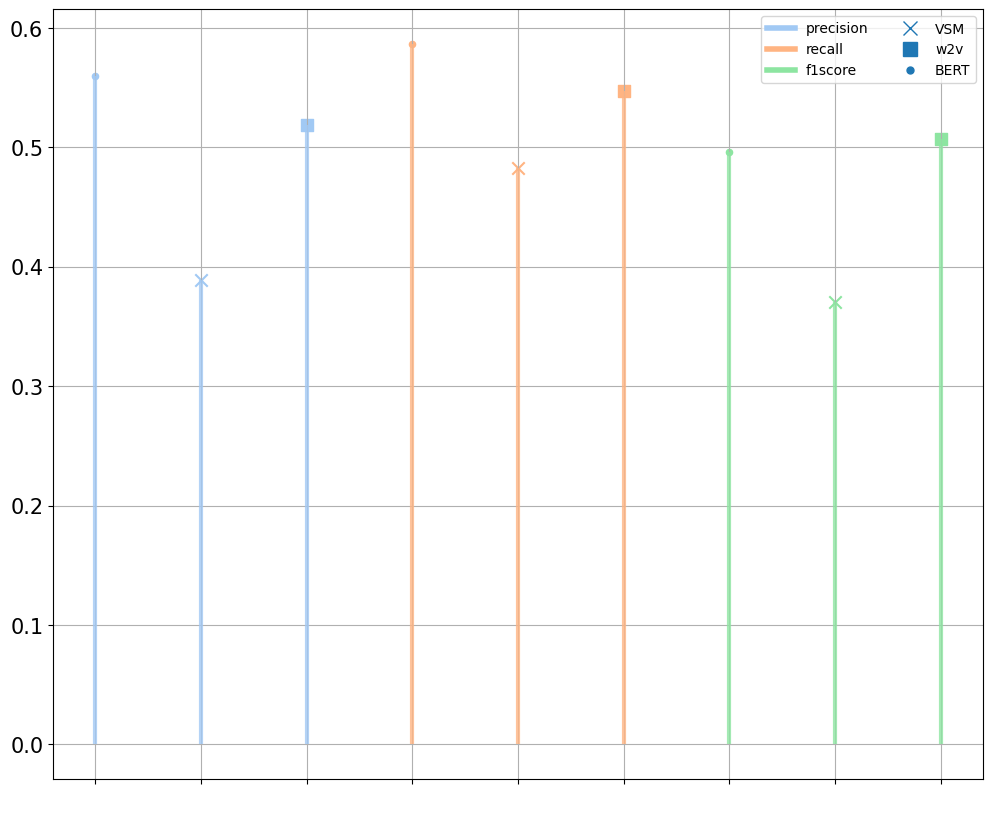
\includegraphics[width=0.95\textwidth]{cp5/results_lollipop}
    \caption{Evaluation results for each technique configuration \red{Draft: I will split the figure in 3. One for each metric. The markers will represent the filters}}
    % \label{fig:webview-task}
\end{figure}







% \art{Change from tables to plots. Similar to Sarah and Treude~\cite{nadi2020}, show Venn diagram with how many sentences each approach identifies and overlaps between them}
\art{Consider changing from tables to plots.}

\art{I've got all results without seframe filters. This week, filters will be my main focus}

% \begin{table}[H]
\centering    
\begin{small}
\begin{threeparttable}
\begin{tabular}{lcccc}


\textbf{Technique} & 
\textbf{Precision} & \textbf{Recall} & 
\parbox[c][.9cm][c]{1.5cm}{\centering \textbf{Pyramid precision}} & 
\parbox[c][.9cm][c]{1.5cm}{\centering \textbf{Pyramid recall}} \\


\hline


\textbf{word2vec + meaningful-frames} &
0.50 & 0.50 & 
0.50 & 0.50 
\\

\textbf{word2vec + similar-meaning} &
0.50 & 0.50 & 
0.50 & 0.50 
\\


\textbf{BERT + meaningful-frames} &
0.50 & 0.50 & 
0.50 & 0.50 
\\

\textbf{BERT + meaningful-frames} &
0.50 & 0.50 & 
0.50 & 0.50 
\\

\hline

\end{tabular}
\end{threeparttable}
\end{small}
\caption{\art{this can be merged with the previous table}}
\end{table}




% \begin{table}[H]
\centering    
\begin{scriptsize}
\begin{threeparttable}
\begin{tabular}{llcccc}


\textbf{} & \textbf{Technique} &
\textbf{Precision} & \textbf{Recall} & 
\parbox[c][.7cm][c]{1.5cm}{\centering \textbf{Pyramid precision}} & 
\parbox[c][.7cm][c]{1.5cm}{\centering \textbf{Pyramid recall}} \\


\hline

\multirow{ 2}{*}{\textbf{Baseline}}  & VSM &
0.50 & 0.50 & 
0.50 & 0.50 
\\

& ours &
0.50 & 0.50 & 
0.50 & 0.50 
\\

\hline

\multirow{ 2}{*}{\textbf{API documentation}}  & Kreck &
0.50 & 0.50 & 
0.50 & 0.50 
\\

& ours &
0.50 & 0.50 & 
0.50 & 0.50 
\\

\hline

\multirow{ 2}{*}{\textbf{GitHub issues}} & Hurried &
0.50 & 0.50 & 
0.50 & 0.50 
\\

 & Ours &
0.50 & 0.50 & 
0.50 & 0.50 
\\

\hline

\multirow{ 2}{*}{\textbf{SO answers}} & AnsBot &
0.50 & 0.50 & 
0.50 & 0.50 
\\

 & Ours &
0.50 & 0.50 & 
0.50 & 0.50 
\\

\hline

\end{tabular}
\end{threeparttable}
\end{scriptsize}
\caption{Techniques comparison}
\label{tbl:approach-results-artifacts}
\end{table}








